%%
% Copyright (c) 2017 - 2020, Pascal Wagler;
% Copyright (c) 2014 - 2020, John MacFarlane
%
% All rights reserved.
%
% Redistribution and use in source and binary forms, with or without
% modification, are permitted provided that the following conditions
% are met:
%
% - Redistributions of source code must retain the above copyright
% notice, this list of conditions and the following disclaimer.
%
% - Redistributions in binary form must reproduce the above copyright
% notice, this list of conditions and the following disclaimer in the
% documentation and/or other materials provided with the distribution.
%
% - Neither the name of John MacFarlane nor the names of other
% contributors may be used to endorse or promote products derived
% from this software without specific prior written permission.
%
% THIS SOFTWARE IS PROVIDED BY THE COPYRIGHT HOLDERS AND CONTRIBUTORS
% "AS IS" AND ANY EXPRESS OR IMPLIED WARRANTIES, INCLUDING, BUT NOT
% LIMITED TO, THE IMPLIED WARRANTIES OF MERCHANTABILITY AND FITNESS
% FOR A PARTICULAR PURPOSE ARE DISCLAIMED. IN NO EVENT SHALL THE
% COPYRIGHT OWNER OR CONTRIBUTORS BE LIABLE FOR ANY DIRECT, INDIRECT,
% INCIDENTAL, SPECIAL, EXEMPLARY, OR CONSEQUENTIAL DAMAGES (INCLUDING,
% BUT NOT LIMITED TO, PROCUREMENT OF SUBSTITUTE GOODS OR SERVICES;
% LOSS OF USE, DATA, OR PROFITS; OR BUSINESS INTERRUPTION) HOWEVER
% CAUSED AND ON ANY THEORY OF LIABILITY, WHETHER IN CONTRACT, STRICT
% LIABILITY, OR TORT (INCLUDING NEGLIGENCE OR OTHERWISE) ARISING IN
% ANY WAY OUT OF THE USE OF THIS SOFTWARE, EVEN IF ADVISED OF THE
% POSSIBILITY OF SUCH DAMAGE.
%%

%%
% This is the Eisvogel pandoc LaTeX template.
%
% For usage information and examples visit the official GitHub page:
% https://github.com/Wandmalfarbe/pandoc-latex-template
%%

% Options for packages loaded elsewhere
\PassOptionsToPackage{unicode}{hyperref}
\PassOptionsToPackage{hyphens}{url}
\PassOptionsToPackage{dvipsnames,svgnames*,x11names*,table}{xcolor}
%
\documentclass[
  paper=a4,
  oneside  ,captions=tableheading
]{scrbook}
\usepackage{lmodern}
\usepackage{setspace}
\setstretch{1.2}
\usepackage{amsmath}
\usepackage{ifxetex,ifluatex}
\ifnum 0\ifxetex 1\fi\ifluatex 1\fi=0 % if pdftex
  \usepackage[T1]{fontenc}
  \usepackage[utf8]{inputenc}
  \usepackage{textcomp} % provide euro and other symbols
  \usepackage{amssymb}
\else % if luatex or xetex
  \usepackage{unicode-math}
  \defaultfontfeatures{Scale=MatchLowercase}
  \defaultfontfeatures[\rmfamily]{Ligatures=TeX,Scale=1}
\fi
% Use upquote if available, for straight quotes in verbatim environments
\IfFileExists{upquote.sty}{\usepackage{upquote}}{}
\IfFileExists{microtype.sty}{% use microtype if available
  \usepackage[]{microtype}
  \UseMicrotypeSet[protrusion]{basicmath} % disable protrusion for tt fonts
}{}
\makeatletter
\@ifundefined{KOMAClassName}{% if non-KOMA class
  \IfFileExists{parskip.sty}{%
    \usepackage{parskip}
  }{% else
    \setlength{\parindent}{0pt}
    \setlength{\parskip}{6pt plus 2pt minus 1pt}}
}{% if KOMA class
  \KOMAoptions{parskip=half}}
\makeatother
\usepackage{xcolor}
\definecolor{default-linkcolor}{HTML}{A50000}
\definecolor{default-filecolor}{HTML}{A50000}
\definecolor{default-citecolor}{HTML}{4077C0}
\definecolor{default-urlcolor}{HTML}{4077C0}
\IfFileExists{xurl.sty}{\usepackage{xurl}}{} % add URL line breaks if available
\IfFileExists{bookmark.sty}{\usepackage{bookmark}}{\usepackage{hyperref}}
\hypersetup{
  pdftitle={Appunti Programmazione 1 - Riccardi},
  pdfauthor={Giovanni Foletto; Enrico Carnelos; Stefano Viel},
  hidelinks,
  breaklinks=true,
  pdfcreator={LaTeX via pandoc with the Eisvogel template}}
\urlstyle{same} % disable monospaced font for URLs
\usepackage[margin=2.5cm,includehead=true,includefoot=true,centering,]{geometry}
\usepackage{listings}
\newcommand{\passthrough}[1]{#1}
\lstset{defaultdialect=[5.3]Lua}
\lstset{defaultdialect=[x86masm]Assembler}
% add backlinks to footnote references, cf. https://tex.stackexchange.com/questions/302266/make-footnote-clickable-both-ways
\usepackage{footnotebackref}
\usepackage{graphicx}
\makeatletter
\def\maxwidth{\ifdim\Gin@nat@width>\linewidth\linewidth\else\Gin@nat@width\fi}
\def\maxheight{\ifdim\Gin@nat@height>\textheight\textheight\else\Gin@nat@height\fi}
\makeatother
% Scale images if necessary, so that they will not overflow the page
% margins by default, and it is still possible to overwrite the defaults
% using explicit options in \includegraphics[width, height, ...]{}
\setkeys{Gin}{width=\maxwidth,height=\maxheight,keepaspectratio}
% Set default figure placement to htbp
\makeatletter
\def\fps@figure{htbp}
\makeatother
\setlength{\emergencystretch}{3em} % prevent overfull lines
\providecommand{\tightlist}{%
  \setlength{\itemsep}{0pt}\setlength{\parskip}{0pt}}
\setcounter{secnumdepth}{-\maxdimen} % remove section numbering

% Make use of float-package and set default placement for figures to H.
% The option H means 'PUT IT HERE' (as  opposed to the standard h option which means 'You may put it here if you like').
\usepackage{float}
\floatplacement{figure}{H}

\ifluatex
  \usepackage{selnolig}  % disable illegal ligatures
\fi

\title{Appunti Programmazione 1 - Riccardi}
\author{Giovanni Foletto \and Enrico Carnelos \and Stefano Viel}
\date{2020-11-21}



%%
%% added
%%

%
% language specification
%
% If no language is specified, use English as the default main document language.
%

\ifnum 0\ifxetex 1\fi\ifluatex 1\fi=0 % if pdftex
  \usepackage[shorthands=off,main=english]{babel}
\else
    % Workaround for bug in Polyglossia that breaks `\familydefault` when `\setmainlanguage` is used.
  % See https://github.com/Wandmalfarbe/pandoc-latex-template/issues/8
  % See https://github.com/reutenauer/polyglossia/issues/186
  % See https://github.com/reutenauer/polyglossia/issues/127
  \renewcommand*\familydefault{\sfdefault}
    % load polyglossia as late as possible as it *could* call bidi if RTL lang (e.g. Hebrew or Arabic)
  \usepackage{polyglossia}
  \setmainlanguage[]{english}
\fi



%
% for the background color of the title page
%
\usepackage{pagecolor}
\usepackage{afterpage}
\usepackage{tikz}
\usepackage[margin=2.5cm,includehead=true,includefoot=true,centering]{geometry}

%
% break urls
%
\PassOptionsToPackage{hyphens}{url}

%
% When using babel or polyglossia with biblatex, loading csquotes is recommended
% to ensure that quoted texts are typeset according to the rules of your main language.
%
\usepackage{csquotes}

%
% captions
%
\definecolor{caption-color}{HTML}{777777}
\usepackage[font={stretch=1.2}, textfont={color=caption-color}, position=top, skip=4mm, labelfont=bf, singlelinecheck=false, justification=raggedright]{caption}
\setcapindent{0em}

%
% blockquote
%
\definecolor{blockquote-border}{RGB}{221,221,221}
\definecolor{blockquote-text}{RGB}{119,119,119}
\usepackage{mdframed}
\newmdenv[rightline=false,bottomline=false,topline=false,linewidth=3pt,linecolor=blockquote-border,skipabove=\parskip]{customblockquote}
\renewenvironment{quote}{\begin{customblockquote}\list{}{\rightmargin=0em\leftmargin=0em}%
\item\relax\color{blockquote-text}\ignorespaces}{\unskip\unskip\endlist\end{customblockquote}}

%
% Source Sans Pro as the de­fault font fam­ily
% Source Code Pro for monospace text
%
% 'default' option sets the default
% font family to Source Sans Pro, not \sfdefault.
%
\ifnum 0\ifxetex 1\fi\ifluatex 1\fi=0 % if pdftex
    \usepackage[default]{sourcesanspro}
  \usepackage{sourcecodepro}
  \else % if not pdftex
    \usepackage[default]{sourcesanspro}
  \usepackage{sourcecodepro}

  % XeLaTeX specific adjustments for straight quotes: https://tex.stackexchange.com/a/354887
  % This issue is already fixed (see https://github.com/silkeh/latex-sourcecodepro/pull/5) but the
  % fix is still unreleased.
  % TODO: Remove this workaround when the new version of sourcecodepro is released on CTAN.
  \ifxetex
    \makeatletter
    \defaultfontfeatures[\ttfamily]
      { Numbers   = \sourcecodepro@figurestyle,
        Scale     = \SourceCodePro@scale,
        Extension = .otf }
    \setmonofont
      [ UprightFont    = *-\sourcecodepro@regstyle,
        ItalicFont     = *-\sourcecodepro@regstyle It,
        BoldFont       = *-\sourcecodepro@boldstyle,
        BoldItalicFont = *-\sourcecodepro@boldstyle It ]
      {SourceCodePro}
    \makeatother
  \fi
  \fi

%
% heading color
%
\definecolor{heading-color}{RGB}{40,40,40}
\addtokomafont{section}{\color{heading-color}}
% When using the classes report, scrreprt, book,
% scrbook or memoir, uncomment the following line.
%\addtokomafont{chapter}{\color{heading-color}}

%
% variables for title, author and date
%
\usepackage{titling}
\title{Appunti Programmazione 1 - Riccardi}
\author{Giovanni Foletto, Enrico Carnelos, Stefano Viel}
\date{2020-11-21}

%
% tables
%

%
% remove paragraph indention
%
\setlength{\parindent}{0pt}
\setlength{\parskip}{6pt plus 2pt minus 1pt}
\setlength{\emergencystretch}{3em}  % prevent overfull lines

%
%
% Listings
%
%


%
% general listing colors
%
\definecolor{listing-background}{HTML}{F7F7F7}
\definecolor{listing-rule}{HTML}{B3B2B3}
\definecolor{listing-numbers}{HTML}{B3B2B3}
\definecolor{listing-text-color}{HTML}{000000}
\definecolor{listing-keyword}{HTML}{435489}
\definecolor{listing-keyword-2}{HTML}{1284CA} % additional keywords
\definecolor{listing-keyword-3}{HTML}{9137CB} % additional keywords
\definecolor{listing-identifier}{HTML}{435489}
\definecolor{listing-string}{HTML}{00999A}
\definecolor{listing-comment}{HTML}{8E8E8E}

\lstdefinestyle{eisvogel_listing_style}{
  language         = java,
  numbers          = left,
  xleftmargin      = 2.7em,
  framexleftmargin = 2.5em,
  backgroundcolor  = \color{listing-background},
  basicstyle       = \color{listing-text-color}\linespread{1.0}\small\ttfamily{},
  breaklines       = true,
  frame            = single,
  framesep         = 0.19em,
  rulecolor        = \color{listing-rule},
  frameround       = ffff,
  tabsize          = 4,
  numberstyle      = \color{listing-numbers},
  aboveskip        = 1.0em,
  belowskip        = 0.1em,
  abovecaptionskip = 0em,
  belowcaptionskip = 1.0em,
  keywordstyle     = {\color{listing-keyword}\bfseries},
  keywordstyle     = {[2]\color{listing-keyword-2}\bfseries},
  keywordstyle     = {[3]\color{listing-keyword-3}\bfseries\itshape},
  sensitive        = true,
  identifierstyle  = \color{listing-identifier},
  commentstyle     = \color{listing-comment},
  stringstyle      = \color{listing-string},
  showstringspaces = false,
  escapeinside     = {/*@}{@*/}, % Allow LaTeX inside these special comments
  literate         =
  {á}{{\'a}}1 {é}{{\'e}}1 {í}{{\'i}}1 {ó}{{\'o}}1 {ú}{{\'u}}1
  {Á}{{\'A}}1 {É}{{\'E}}1 {Í}{{\'I}}1 {Ó}{{\'O}}1 {Ú}{{\'U}}1
  {à}{{\`a}}1 {è}{{\'e}}1 {ì}{{\`i}}1 {ò}{{\`o}}1 {ù}{{\`u}}1
  {À}{{\`A}}1 {È}{{\'E}}1 {Ì}{{\`I}}1 {Ò}{{\`O}}1 {Ù}{{\`U}}1
  {ä}{{\"a}}1 {ë}{{\"e}}1 {ï}{{\"i}}1 {ö}{{\"o}}1 {ü}{{\"u}}1
  {Ä}{{\"A}}1 {Ë}{{\"E}}1 {Ï}{{\"I}}1 {Ö}{{\"O}}1 {Ü}{{\"U}}1
  {â}{{\^a}}1 {ê}{{\^e}}1 {î}{{\^i}}1 {ô}{{\^o}}1 {û}{{\^u}}1
  {Â}{{\^A}}1 {Ê}{{\^E}}1 {Î}{{\^I}}1 {Ô}{{\^O}}1 {Û}{{\^U}}1
  {œ}{{\oe}}1 {Œ}{{\OE}}1 {æ}{{\ae}}1 {Æ}{{\AE}}1 {ß}{{\ss}}1
  {ç}{{\c c}}1 {Ç}{{\c C}}1 {ø}{{\o}}1 {å}{{\r a}}1 {Å}{{\r A}}1
  {€}{{\EUR}}1 {£}{{\pounds}}1 {«}{{\guillemotleft}}1
  {»}{{\guillemotright}}1 {ñ}{{\~n}}1 {Ñ}{{\~N}}1 {¿}{{?`}}1
  {…}{{\ldots}}1 {≥}{{>=}}1 {≤}{{<=}}1 {„}{{\glqq}}1 {“}{{\grqq}}1
  {”}{{''}}1
}
\lstset{style=eisvogel_listing_style}

%
% Java (Java SE 12, 2019-06-22)
%
\lstdefinelanguage{Java}{
  morekeywords={
    % normal keywords (without data types)
    abstract,assert,break,case,catch,class,continue,default,
    do,else,enum,exports,extends,final,finally,for,if,implements,
    import,instanceof,interface,module,native,new,package,private,
    protected,public,requires,return,static,strictfp,super,switch,
    synchronized,this,throw,throws,transient,try,volatile,while,
    % var is an identifier
    var
  },
  morekeywords={[2] % data types
    % primitive data types
    boolean,byte,char,double,float,int,long,short,
    % String
    String,
    % primitive wrapper types
    Boolean,Byte,Character,Double,Float,Integer,Long,Short
    % number types
    Number,AtomicInteger,AtomicLong,BigDecimal,BigInteger,DoubleAccumulator,DoubleAdder,LongAccumulator,LongAdder,Short,
    % other
    Object,Void,void
  },
  morekeywords={[3] % literals
    % reserved words for literal values
    null,true,false,
  },
  sensitive,
  morecomment  = [l]//,
  morecomment  = [s]{/*}{*/},
  morecomment  = [s]{/**}{*/},
  morestring   = [b]",
  morestring   = [b]',
}

\lstdefinelanguage{XML}{
  morestring      = [b]",
  moredelim       = [s][\bfseries\color{listing-keyword}]{<}{\ },
  moredelim       = [s][\bfseries\color{listing-keyword}]{</}{>},
  moredelim       = [l][\bfseries\color{listing-keyword}]{/>},
  moredelim       = [l][\bfseries\color{listing-keyword}]{>},
  morecomment     = [s]{<?}{?>},
  morecomment     = [s]{<!--}{-->},
  commentstyle    = \color{listing-comment},
  stringstyle     = \color{listing-string},
  identifierstyle = \color{listing-identifier}
}

%
% header and footer
%
\usepackage{fancyhdr}

\fancypagestyle{eisvogel-header-footer}{
  \fancyhead{}
  \fancyfoot{}
  \lhead[2020-11-21]{Appunti Programmazione 1 - Riccardi}
  \chead[]{}
  \rhead[Appunti Programmazione 1 - Riccardi]{2020-11-21}
  \lfoot[\thepage]{Giovanni Foletto, Enrico Carnelos, Stefano Viel}
  \cfoot[]{}
  \rfoot[Giovanni Foletto, Enrico Carnelos, Stefano Viel]{\thepage}
  \renewcommand{\headrulewidth}{0.4pt}
  \renewcommand{\footrulewidth}{0.4pt}
}
\pagestyle{eisvogel-header-footer}

%%
%% end added
%%

\begin{document}

%%
%% begin titlepage
%%
\begin{titlepage}
\newgeometry{top=2cm, right=4cm, bottom=3cm, left=4cm}
\tikz[remember picture,overlay] \node[inner sep=0pt] at (current page.center){
\includegraphics[width=\paperwidth,height=\paperheight]{./image/background.pdf}};
\newcommand{\colorRule}[3][black]{\textcolor[HTML]{#1}{\rule{#2}{#3}}}
\begin{flushleft}
\noindent
\\[-1em]
\color[HTML]{FFFFFF}
\makebox[0pt][l]{\colorRule[360049]{1.3\textwidth}{0pt}}
\par
\noindent

% The titlepage with a background image has other text spacing and text size
{
  \setstretch{2}
  \vfill
  \vskip -8em
  \noindent {\huge \textbf{\textsf{Appunti Programmazione 1 -
Riccardi}}}
    \vskip 2em
  \noindent {\Large \textsf{Giovanni Foletto, Enrico Carnelos, Stefano
Viel} \vskip 0.6em \textsf{2020-11-21}}
  \vfill
}


\end{flushleft}
\end{titlepage}
\restoregeometry

%%
%% end titlepage
%%



Giovanni Foletto, Stefano Viel, Carnelos Enrico - Primo anno ICE

\hypertarget{programmazione-1---riccardi}{%
\section{PROGRAMMAZIONE 1 -
RICCARDI}\label{programmazione-1---riccardi}}

\hypertarget{lezioni-teoriche}{%
\subsection{Lezioni teoriche}\label{lezioni-teoriche}}

\hypertarget{obiettivi-e-cosuxe8-linformatica}{%
\subsubsection{0.0) Obiettivi e Cos'è
l'informatica:}\label{obiettivi-e-cosuxe8-linformatica}}

\hspace{0pt} \textbf{Obiettivo}: conoscenza di base dell'informatica.

\hspace{0pt} \textbf{Informatica}: dal francese, informazione
automatica. Termine coniato da Ph. Dreyfus nel 1962

\hspace{0pt} Questo significa che è l'insieme degli aspetti scientifici
e tecnici che sono specificatamente applicati alla raccolta e al
trattamento dell'informazione, in particolare all'elaborazione
automatica dei dai. Ma anche lo studio sistematico degli algoritmi che
descrivono e trasformano l'informazione.

\hypertarget{algoritmi-e-linguaggi-di-programmazione}{%
\subsubsection{1.1) Algoritmi e linguaggi di
programmazione:}\label{algoritmi-e-linguaggi-di-programmazione}}

Un \textbf{algoritmo} è una sequenza precisa di operazioni,
comprensibili da un esecutore, che definisce una sequenza finita di
passi che portano alla realizzazione di un compito (\emph{task o
problema}).

L'algoritmo ha alcune caratteristiche: (2 e 3 sono le più importanti)

\begin{enumerate}
\def\labelenumi{\arabic{enumi}.}
\tightlist
\item
  deve essere \textbf{comprensibile} al suo esecutore (linguaggi di
  programmazione nel caso di un calcolatore). L'algoritmo così
  codificato viene chiamato \emph{programma}.
\item
  deve essere \textbf{corretto } (l'algoritmo ottiene la soluzione del
  compito cui è preposto, senza errori in nessun passo fondamentale).
\item
  deve essere \textbf{efficente} (l'algoritmo ottiene la soluzione
  usando la minor quantità di risorse).
\end{enumerate}

DA NOTARE CHE: il concetto di algoritmo non è prerogativa dei
calcolatori, ma semplicemente il calcolatore (in questo caso un
computer) ha capacità di calcolo tali da gestire e lavorare con quantità
di dati altrimenti intrattabili.

Gli algoritmi sono il modo in cui, implicitamente o esplicitamente,
affrontiamo ogni problema nella vita di tutti i giorni. Questo problema
viene chiamato \textbf{task}, e l'algoritmo serve a risolverlo.

Il problema dell'algoritmo della scelta invece crea un problema, il
cosiddetto \textbf{il problema della segretaria}, che contiene una
semplificazione matematica dell'algoritmo della scelta ottimale dal
punto di vista matematico.

Il concetto di questo problema è che dovendo scegliere di assumere una
tra 100 segretarie, con l'unica remora che una volta assunta una, non si
continua a cercare. L'algoritmo in questo caso direbbe di scegliere solo
passati i primi 37\% elementi (in questo caso segretarie), dopodichè,
passato questo step, il primo che si dimostra all'altezza del compito
anche in base alle persone viste in precedenza viene assunto e si chiude
la ricerca.

(Vedi:
https://www.smartworld.it/tecnologia/formula-matematica-decisioni-difficili-della-vita.html).

Dal concetto di ottimizzazione e rendimento dell'algoritmo si incontra
anche il concetto di \textbf{reward}: ho due scelte, una usuale
(\textbf{exploit}), un altra che cambia e esce dagli schemi
(\textbf{explore}). La migliore dipende dal migliore risultato che le
due rendono possibile.

\hypertarget{il-grafo}{%
\subparagraph{Il grafo}\label{il-grafo}}

Per la rappresentazione di alcuni logaritmi è molto utile l'utilizzo del
\textbf{grafo}. Il grafo è uno schema che collega tra loro le
informazioni possedute, ottenute anche fonti diverse. Le informazioni
così raccolte hanno il lato positivo di essere facilmente ricercabile,
distinguibile e visibile. Inoltre rende evidenti i collegamenti che
hanno tra loro.

Questo tipo di schematizzazione, essendo molto ottimizzata e mettendo
subito in risalto le informazioni che hanno contatti tra di loro,
vengono ampiamente utilizzati nell'intelligenza artificiale, permettendo
appunto grandi elaborazioni. Il grafo quindi è un oggetto logico molto
potente.

Un accortezza: con questa struttura è facile prendere due grafi uguali
come diversi. I grafi si dicono \textbf{isomorfi} se hanno le stesse
caratteristiche in termini di nodi e archi.

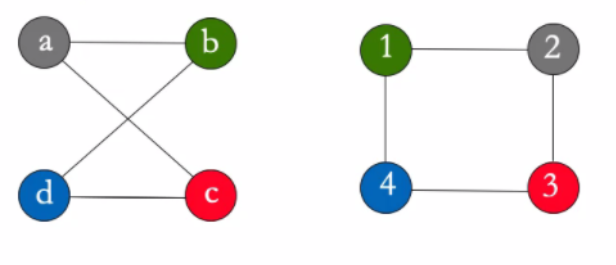
\includegraphics{./image/image-20201110233258123.png}

A questo punto però si crea un problema, infatti in alcuni casi, usando
un dato algoritmo ottengo risultati diversi se non qualifico un qualche
tipo di \textbf{parametro}. Proprio il concetto di parametro (inteso nel
senso informatico, cioè elemento che caratterizza un determinato
algoritmo e che l'algoritmo si aspetta per eseguire un compito). I
parametri quindi possono \textbf{condizionare l'esecuzione del task}.

\hypertarget{come-descrivere-un-algoritmo}{%
\subparagraph{Come descrivere un
algoritmo:}\label{come-descrivere-un-algoritmo}}

L'algoritmo per definizione è una sequenza precisa di passi, di
conseguenza una lista non ordinata di elementi non è l'oggetto giusto
per la sua rappresentazione. Inoltre il fatto che attraverso un
parametro si possa ottenere un risultato diverso rende la sua codifica
difficile.

Innanzitutto è essenziale che sia descritto come un programma, cioè come
una sequenza di istruzioni scritte in un linguaggio comprensibile al
calcolatore. Il compito del programmatore è proprio quello di scrivere
del codice che porti alla soluzione ottimale del problema.

Per iniziare bisogna inizialmente \textbf{definire esattamente il
problema}, che può essere:

\begin{enumerate}
\def\labelenumi{\arabic{enumi}.}
\tightlist
\item
  problema di \textbf{puro calcolo e conversione}, cioè risolvibile
  attraverso conoscenze matematiche.
\item
  problemi di \textbf{decisione}, cioè capire se una certa proprietà è
  propria di un certo elemento. (es. 15467 è primo?).
\item
  problemi di \textbf{ricerca}, cioè trovare un elemento con determinate
  caratteristiche in un determinato insieme.
\end{enumerate}

Il passaggio da definizione del problema a esecuzione del task poi passa
da altri step, che sono necessari alla codifica e alla comprensione dei
vari step:

\begin{enumerate}
\def\labelenumi{\arabic{enumi}.}
\tightlist
\item
  Problema: linguaggio \textbf{Lp}, ovvero linguaggio naturale (per
  descrivere il problema).
\item
  Algoritmo: linguaggio \textbf{La}, ovvero lo pseudocodice (lascia meno
  incomprensione ma più difficile da leggere).
\item
  Programma: linguaggio \textbf{Lt}, ovvero linguaggio macchina (es.
  C/C++).
\end{enumerate}

Una volta eseguiti questi \textbf{macropassaggi} si può passare alla
rifinitura del processo, attraverso dei \textbf{micro-algoritmi} (alcune
volte il programma e l'algoritmo necessario al suo funzionamento sono
così semplici da non necessitare la stesure di micro-algoritmi di
supporto).

Su algoritmi molto complessi si può applicare la tecnica del
\textbf{deconstruct}, ovvero decostruire il problema finché non si
ottengono tanti problemi di facile soluzione.

Nel caso della stesura di un algoritmo si devono prendere in
considerazione tutte le casistiche. Ad esempio se si scrive un algoritmo
per cercare un libro bisogna anche tenere in considerazione la
possibilità che questo libro non sia presente nell'indice della ricerca.
Allo stesso modo non si può pensare di avere una differenza abissale di
prestazioni se il libro è presente nella prima parte di indice o invece
è in fondo. Ci sono di solito sempre più di un modo per risolvere
problemi, quindi il problema principale diventa quello di trovare il
modo più efficiente disponibile.

\hypertarget{la-programmazione-e-il-linguaggio-di-programmazione}{%
\subparagraph{La programmazione e il linguaggio di
programmazione}\label{la-programmazione-e-il-linguaggio-di-programmazione}}

Programmare innanzitutto significa analizzare un problema, progettare un
algoritmo per ottenere una soluzione, esprimere l'algoritmo in un
linguaggio di programmazione, mettere la macchina nella situazione di
eseguire il programma e infine correggere eventuali errori.

L'algoritmo deve essere tradotto da linguaggio formale e reso
comprensibile all'esecutore. L'insieme dei comandi dati al calcolatore
in un certo linguaggio viene chiamato \textbf{programma}.

Il linguaggio di programmazione deve essere \textbf{rigoroso e preciso}
dal punto di vista di:

\begin{enumerate}
\def\labelenumi{\arabic{enumi}.}
\tightlist
\item
  \textbf{sintassi}: le regole che descrivono le stringhe di parole
  riconosciute dal linguaggio.
\item
  \textbf{semantica}: regole per l'interpretazione delle stringhe e che
  descrivono i processi computazionali dell'esecutore (o più
  semplicemente un errore logico nella stesura del programma, cioè un
  errore nella comprensione logica del programma). Questo errore è più
  difficile da individuare perché il compilatore non dà errore, ma i
  risultati saranno incoerenti.
\end{enumerate}

Parlando di linguaggi di programmazione, bisogna dire anche qualcosa
sull'astrazione del linguaggio:

\begin{enumerate}
\def\labelenumi{\arabic{enumi}.}
\item
  se il linguaggio è di bassissimo livello, quindi troppo vicino alla
  macchina è difficile programmare.
\item
  se il linguaggio è troppo di alto livello, quindi molto vicino al
  linguaggio del programmatore, i programmi diventano inefficienti.

  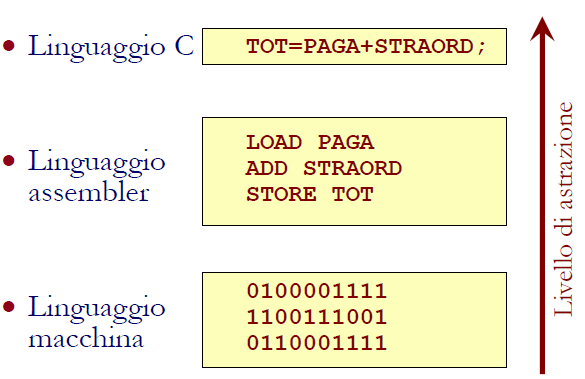
\includegraphics{./image/image-20201111001022024.png}
\end{enumerate}

Agli albori dell'informatica si programmava in linguaggio macchina, cioè
compreso direttamente dalla macchina.

Dagli anni '50 iniziano a nascere i primi linguaggi di programmazione di
alto livello, data la sempre più alta complessità dei programmi.

Ad oggi esistono tantissimi linguaggi di programmazione, ognuno con il
suo scopo e inventato per esigenze diverse.

\hypertarget{metodo-grafico-per-creare-algoritmi}{%
\subparagraph{Metodo grafico per creare
algoritmi:}\label{metodo-grafico-per-creare-algoritmi}}

Gli algoritmi possono essere schematizzati anche attraverso diagrammi di
flusso, cioè blocchi orientati che hanno un significato proprio.

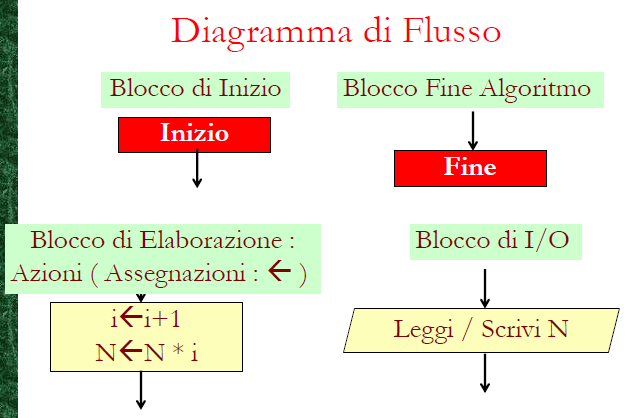
\includegraphics{./image/image-20201111002115408.png}

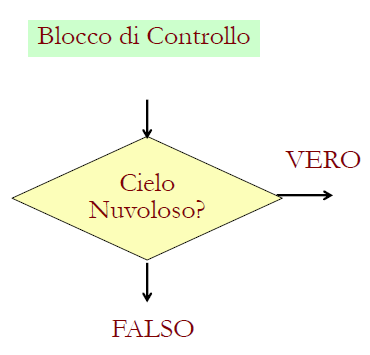
\includegraphics{./image/image-20201111002130617.png}

CARATTERISTICHE:

\begin{itemize}
\tightlist
\item
  BLOCCO \textbf{INIZIO}: unico nodo del grafo da cui si può solo
  partire infatti ha una sola freccia uscente. Rettangolo rosso per
  convenzione. Di solito si definisce con `1' l'inizio.
\item
  BLOCCO \textbf{FINE}: blocco in cui si può solo arrivare infatti ha
  una sola freccia entrante. Rettangoli rossi per convenzione. Di solito
  si definisce con `0' la fine.
\item
  BLOCCO \textbf{ISTRUZIONE}:

  \begin{itemize}
  \tightlist
  \item
    \textbf{assegnazione}: dà il valore che c'è a sinistra alla
    variabile di destra.
  \item
    \textbf{I/O}: (input/output), si sta leggendo o scrivendo
  \item
    \textbf{controllo}: (con più uscite, in questo caso vero e falso)
  \end{itemize}
\end{itemize}

\hypertarget{architettura-hardware-di-un-compilatore}{%
\subsubsection{1.2) Architettura hardware di un
compilatore:}\label{architettura-hardware-di-un-compilatore}}

\hypertarget{storia-del-calcolatore}{%
\subparagraph{Storia del Calcolatore:}\label{storia-del-calcolatore}}

Il primo calcolatore definito tale è ENIAC, creato nel 1945 in America
con il principale scopo di calcolare la traiettoria dell'artiglieria.
Poi donato al University of Pennsylvania, dove invece venne usato per il
calcolo ingegneristico e scientifico. Pesava circa 27 tonnellate e per
programmarlo erano necessarie diverse persone, infatti si basava su una
\emph{plugbboard} cioè un sistema di ``prese'' che, usate per fare il
contatto giusto, fornivano risultati alle operazioni date come input.
Non esisteva un linguaggio di programmazione pe questo computer e i
cosiddetti ``programmatori'' dell'epoca probabilmente non lo hanno mai
visto in tutta la loro vita, dato che loro facevano solo i calcoli per
farlo funzionare e poi qualcun altro si occupava di creare i giusti
collegamenti. La sua potenza di calcolo era tale da permettere di
calcolare quello che un uomo avrebbe fatto in 20 ore in soli 30 secondi.
Aveva un clock di circa 100kHz, e garantiva una vasta quantità di
calcoli possibili.

Dopo la seconda guerra mondiale inizia effettivamente lo sviluppo di una
macchina più vicina all'immaginari comune. Sempre più comuni diventano:

\begin{enumerate}
\def\labelenumi{\arabic{enumi}.}
\tightlist
\item
  MAINFRAME: computer di grandi dimensioni ed elevata potenza,
  solitamente condiviso fra più persone/uffici.
\item
  PERSONAL COMPUTER: computer dotati di tastiera e schermo separati, di
  memoria di massa interni o esterni alla memoria centrale e molto più
  economico.
\item
  LAPTOP: computer portatile, nonché evoluzione portabile del personal
  computer. Diventa molto famoso e utilizzato. Diventano così
  sofisticati che inizia il processo di miniaturizzazione dato che si
  poteva fare con le tecnologie disponibili ormai.
\item
  HANDHELD COMPUTER (SMARTPHONE): cellulari dotati di touchscreen, molto
  portabili e maneggevoli. Anche con questi come con i laptop avviene il
  processo di miniaturizzazione.
\item
  WHERABLE COMPUTER: sono computer così miniaturizzati da poter essere
  messi all'interno di un orologio, o un altro oggetto facilmente
  indossabile. Questi solamente sono caratterizzati da una gamma di
  sensori solitamente molto avanzati che possono servire per monitorare
  lo stato di salute o altri scopi.
\end{enumerate}

La miniaturizzazione che è avvenuta è dovuta alla possibilità di
dimezzare la grandezza del transistor per un certa quantità di volte,
data dalla legge di Moore.

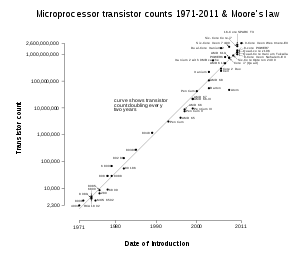
\includegraphics{./image/290px-Transistor_Count_and_Moore's_Law_-_2011.svg.png}

Moore infatti nel 1965 ipotizza che il numero di transistor inseribili
nei microprocessori sarebbe raddoppiato ogni anno. La sua previsione si
rivela corretta, finché verso la fine degli anni '80 viene riformulata:
raddoppio del numero di transistori ogni 18 mesi.

Per aumentare ancora più le prestazioni si cerca di aumentare il clock
dei processori stessi. Il \textbf{clock} di un processore è il dato che
indica la quantità di calcoli può fare al secondo. Al momento il dato
del clock è pressoché fermo intorno al dato di 3gHz. Questo stop è
dovuto al problema fisico per cui aumentando troppo il clock, il calore
emesso diventa esponenzialmente maggiore. Di conseguenza quando si sono
provati clock più alti si ha avuto problemi di gestione delle
temperature eccessivamente alte. Per ovviare questo problema si apre
un'altra strada: il multithreading o clock distribuito ad albero. Questo
permette di passare il clock in tutte le parti del processore e rendere
quindi i processi sincronizzati, utilizzando la potenza di tutte le
parti assieme e quindi garantendo una maggior potenza.

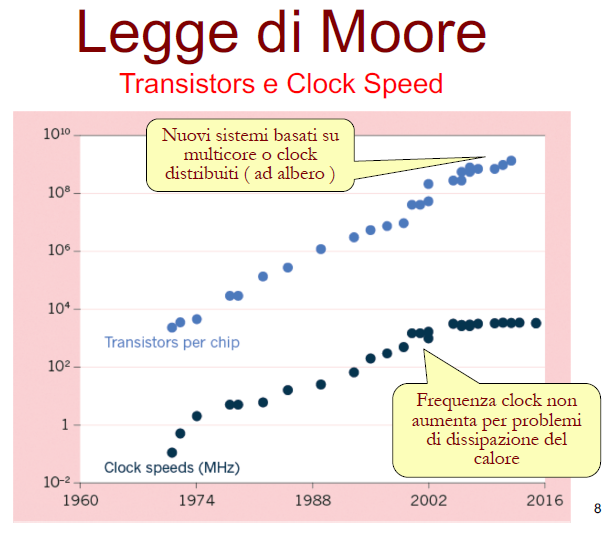
\includegraphics{./image/image-20201111171947392.png}

\hypertarget{organizzare-il-software-di-un-calcolatore}{%
\subparagraph{Organizzare il software di un
calcolatore}\label{organizzare-il-software-di-un-calcolatore}}

Il normale schema di un calcolatore è (generalmente) così costruito:

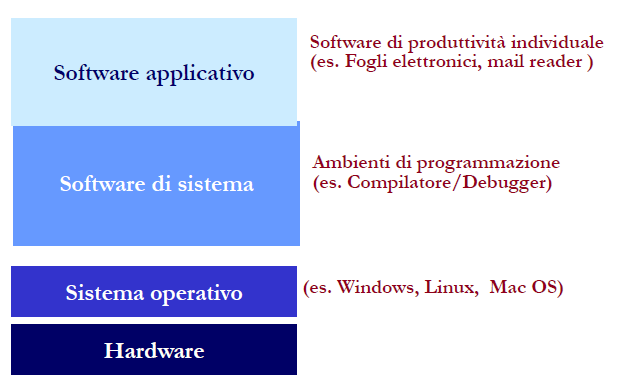
\includegraphics{./image/image-20201111172243268.png}

Per leggere questo schema bisogna capire che:

\begin{enumerate}
\def\labelenumi{\arabic{enumi}.}
\tightlist
\item
  Tutto si basa su quello che ha sotto di se e può comunicare solo con i
  blocchi a se adiacenti. (ad es. il software di sistema non si
  interfaccia direttamente con l'hardware, passa attraverso il sistema
  operativo).
\item
  L'unico che può operare con l'hardware è il sistema operativo. Questo
  ne gestisce tutte le componenti.
\end{enumerate}

\hypertarget{architettura-hardware}{%
\subparagraph{Architettura Hardware:}\label{architettura-hardware}}

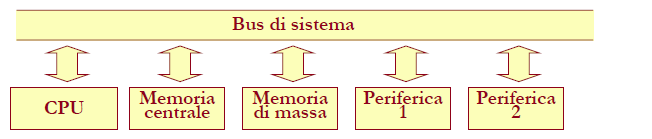
\includegraphics{./image/image-20201111172642835.png}

L'architettura hardware sopra è nota con il nome di \textbf{Macchina di
Von Neumann} ed è così costituita:

\begin{enumerate}
\def\labelenumi{\arabic{enumi}.}
\tightlist
\item
  \textbf{CPU} (central processing unit): svolge l'elaborazione
  eseguendo i programmi logici.
\item
  \textbf{MEMORIA CENTRALE }: memoria utilizzata per memorizzare dati e
  istruzioni, volatile (usata quindi solo per l'esecuzione di
  programmi).
\item
  \textbf{MEMORIA DI MASSA }: usata per memorizzare grandi quantità di
  dati e programmi in maniera persistente, al contrario della memoria
  centrale.
\item
  \textbf{PERIFERICHE}: sono di vario tipo e servono a tutto quello che
  permette l'interazione con il calcolatore. (ad es. tastiera, monitor,
  stampante, ..).
\item
  \textbf{BUS DI SISTEMA}: elemento che interconnette gli altri
  componenti consentendo lo scambio di dati, quindi anche il
  collegamento fra periferiche e hardware.
\end{enumerate}

\hypertarget{macchina-di-von-neumann}{%
\subparagraph{Macchina di Von Neumann:}\label{macchina-di-von-neumann}}

1.2.1) CPU: unità di elaborazione

La CPU è l'unità di elaborazione del calcolatore, si occupa di caricare
le istruzioni in memoria centrale, interpretarle e eseguirle.

E' altamente specializzata, perché è pensata per eseguire pochi tipi di
operazioni ma molto velocemente.

Il suo lavoro è scandito dal \textbf{clock} (orologio interno). La
potenza del calcolatore dipende in parte dal clock, infatti quanto più
questo è alto, tante più sono le istruzioni che riesce ad eseguire al
secondo. La sua frequenza infatti viene misurata in Hz, e 1 Hz = 1
ciclo/s. Ad oggi le CPU riescono a lavorare in parallelo, il cosiddetto
``lavoro condiviso'', grazie al clock. Infatti il segnale del clock che
arriva a tutti sincronizzato permette di eseguire azioni
contemporaneamente.

1.2.2) Memoria centrale:

La memoria centrale è destinata a accogliere dati e programmi sui quali
opera il calcolatore. (ad es. quando usiamo il computer qui vengono
memorizzati i dati di programmi che stiamo usando, \ldots). La memoria
centrale è velocissima ma volatile (cioè una volta che il programma
finisce, tutti i dati di un programma vengono cancellati e lo spazio
viene liberato). Questa memoria accoglie i dati necessari a far
funzionare i programmi. Concettualmente è composta da una sequenza di
celle ognuna delle quali contiene una parola (\textbf{word}). Ad ogni
cella si può accedere direttamente specificandone l'\textbf{indirizzo},
e accedendone si può cambiare il suo contenuto (read/write). La quantità
di bit da cui è composta la word dipende dalla macchina, infatti è
caratteristico del microprocessore e attraverso questo si identifica lo
spazio di indirizzamento.

La memoria centrale solitamente è realizzata da una \textbf{RAM} (random
access memory). La sua caratteristica è che ogni cosa è accessibile e
non devo scansionare tutti gli indirizzi per cercare la cella che ho
bisogno. (per es. non è come il nastro magnetico che devono fisicamente
essere spostate avanti e indietro per trovare l'informazione cercata).
Questo ha ricadute dirette sul tempo di accesso, che è indipendente
dall'indirizzo della word che si vuole accedere. Questa è una memoria
volatile quindi i dati presenti qui sopra si perdono quando si spegne la
macchina. Esistono SRAM (static RAM), molto veloce, può contenere pochi
dati acceduti molto frequentemente, e DRAM (dynamic RAM) che contiene
più dati, ma più lentamente.

Altri tipi di memoria presenti sono le \textbf{ROM} (read-only memory).
Hanno caratteristiche simile alle RAM, hanno un accesso veloce ai dati
(ma non come quello delle RAM) e si tratta di \textbf{memorie
permanenti} su cui però non si può scrivere. Tipicamente son utilizzate
per memorizzare dati e programmi che servono prima del caricamento del
Sistema Operativo (ad es. per il caricamento del BIOS = Basic
Input-Output System).

La memoria quindi com'è fatta? Appare come una lista di word cioè un
mattoncino composto da 16bit, di conseguenza posso memorizzare tanti dai
quanti 2\^{}16 valori binari. All'interno della memoria ci posso mettere
tante word come gli indirizzi di memoria che sono 1024, e sono assegnati
da 0 a 1023. Se questi fossero i limiti del tuo microprocessore allora
devi fare in modo che all'interno di questo spazio di memoria ci stiano
i dati e i programmi necessari al tuo scopo.

Per questo motivo in memoria non si può accedere a valori più grandi di
2\^{}16 e non si può accedere all'indirizzo 1024.

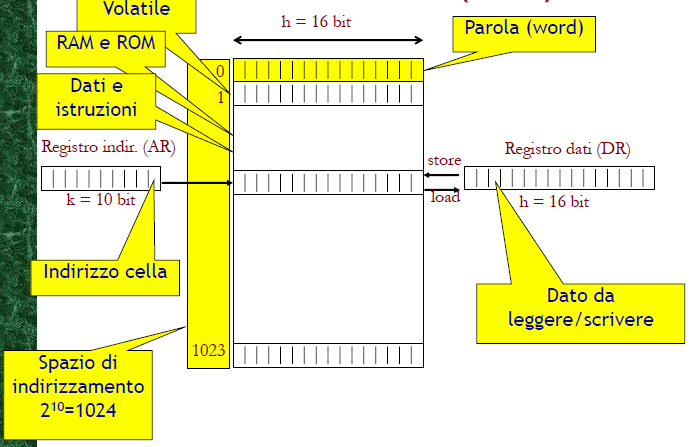
\includegraphics{./image/image-20201111185631084.png}

Però poi a questa memoria si deve poter accedere, quindi nella CPU
esistono dei registri, che sono word di memoria chiamate così per
distinguerle da quelle in memoria centrale. Questi registri possono
essere:

\begin{enumerate}
\def\labelenumi{\arabic{enumi}.}
\tightlist
\item
  AR (Address Register): di almeno 10 bit, perché in questo caso posso
  indirizzare da 0 a 1023
\item
  DR (data Register): posto in cui i dati di cui la CPU ha bisogno per
  fare operazioni che vengono copiati in questa posizione dalla memoria
  centrale per rendere le informazioni direttamente disponibili alla
  CPU.
\end{enumerate}

I registri sono elementi di supporto al calcolo.

1.2.3) Gerarchia di memoria

Ci sono a disposizione memorie con caratteristiche diverse in base al
loro scopo:

\begin{enumerate}
\def\labelenumi{\arabic{enumi}.}
\tightlist
\item
  Registri: presenti nella CPU, piccoli ma veloci, utili per contenere
  dati temporanei per le operazioni della CPU
\item
  Memoria cache (SRAM): veloce, contiene pochi dati usati/richiesti
  frequentemente
\item
  Memoria principale (DRAM): meno veloce ma contiene più dati
\item
  Memoria secondaria o di Massa: molti dati, indicativamente più lenti
  (anche se gli SSD consentono un vantaggio prestazionale rispetto agli
  HD o agli HHD).
\end{enumerate}

1.2.4) Rappresentazione dell'informazione:

Tutti i dati vengono solitamente rappresentati in maniera
\textbf{binaria}, ovvero il bit che può prendere il valore 0 o 1. Questo
è molto utile perché si basano strutturalmente basati su dispositivi
bistabili (corrente ON o corrente OFF). Per questo l'elaboratore
elettronico può operare solo su sequenze di simboli binari.

Il BIT (derivato da Bynary digIT) è quindi l'unità elementare
dell'informazione. Comandi e dati nel computer vengono quindi
rappresentati con lunghe sequenze di numeri binari.

Essendo tutto codificabile attraverso il bit, allora sono state
inventate strutture per contenere la rappresentazione figurata della
realtà. Ad esempio la convenzione ASCII, poi diventata extended-ASCII,
ha codificato i caratteri come sequenza di 8bit, il \textbf{byte}.

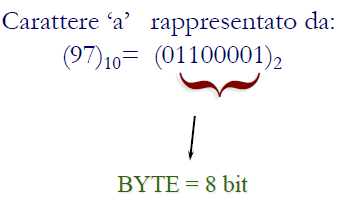
\includegraphics{./image/image-20201111184647324.png}

Per i multipli del byte si adottano gli stessi simboli del sistema
decimale, ma visto che gli elementi sono in base 2, il fattore di scala
è leggermente diverso:

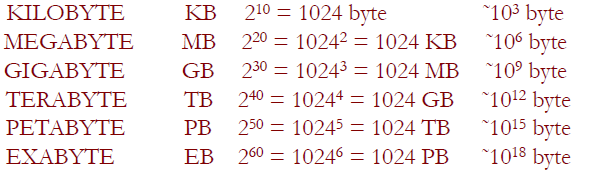
\includegraphics{./image/image-20201111184937248.png}

1.2.5) Funzionamento della CPU:

Innanzitutto bisogna dire che:

\begin{enumerate}
\def\labelenumi{\arabic{enumi}.}
\tightlist
\item
  il trasferimento dei dati avviene con il bus di sistema.
\item
  Le fasi di elaborazione si susseguono in modo sincrono rispetto
  all'orologio di sistema (clock).
\item
  Durante ogni intervallo di tempo \textbf{l'unità di controllo} (che fa
  parte del processore) stabilisce la funzione da svolgere.
\item
  L'intera macchina opera in maniera sequenziale (però architetture più
  evolute prevedono l'esecuzione parallela delle istruzioni).
\end{enumerate}

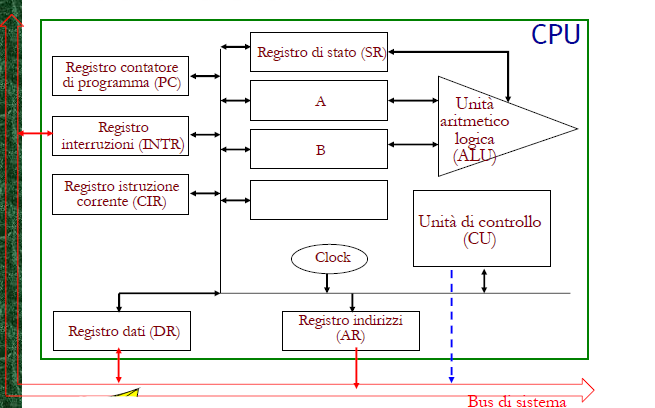
\includegraphics{./image/image-20201111191808017.png}

Come si vede dall'immagine la CPU ha a disposizione vari elementi:

\begin{enumerate}
\def\labelenumi{\arabic{enumi}.}
\tightlist
\item
  i registri (PC, INTR, CIR, DR, AR, \ldots)

  \begin{itemize}
  \tightlist
  \item
    registro di stato della CPU (\textbf{SR})(FLAG: C, Z, S, V), serve a
    far capire al compilatore lo stato delle periferiche e delle varie
    parti del compilatore stesso.
  \item
    Il program counter (\textbf{PC}) indica gli indirizzi dove andare a
    prendere la prossima istruzione.
  \item
    registro istruzioni (\textbf{INTR}) segnale lo stato di
    funzionamento delle periferiche.
  \end{itemize}
\item
  unità di controllo: capacità di controllare quello che sta succedendo,
  in pratica manda segnali per impartire degli ordini, in particolare
  possono provenire da questa unità il segnale di prelievo, di
  decodifica e d'esecuzione dell'istruzione.
\item
  Unità ALO: oggetto che esegue le operazioni aritmetico-logiche.
\item
  si nota il BUS di SISTEMA, responsabile di collegarsi ai vari registri
  e alle varie periferiche. (sotto)
\end{enumerate}

Il Ciclo base di funzionamento della CPU: (visione ad alto livello)

\begin{enumerate}
\def\labelenumi{\arabic{enumi}.}
\tightlist
\item
  FETCH

  \begin{enumerate}
  \def\labelenumii{\arabic{enumii}.}
  \tightlist
  \item
    La CU manda un segnale affinché il PC sia spostato nel AR (cioè la
    prossima istruzione viene indicizzata).
  \item
    segnale controllo (read) alla memoria centrale posto all'indirizzo
    in AR.
  \item
    il dato letto viene messo a disposizione nel DR (registro dei dati).
  \item
    la CU manda il segnale di controllo affinché il contenuto di DR sia
    spostato nel CIR (registro istruzione corrente).
  \end{enumerate}
\item
  INTERPRETAZIONE: le informazioni sul CIR vengono decodificate dalla
  CU.
\item
  ESECUZIONE: la CU genera una sequenza di segnali di controllo
  necessari a eseguire l'istruzione.
\item
  il PC viene incrementato per puntare alla prossima istruzione.
\end{enumerate}

Durante l'esecuzione la CPU può eseguire 3 macro-tipologie di
istruzioni:

\begin{enumerate}
\def\labelenumi{\arabic{enumi}.}
\tightlist
\item
  Istruzioni aritmetiche.
\item
  istruzioni di controllo.
\item
  istruzione di trasferimento dei dati (sia registro-registro, sia
  memoria-memoria, sia memoria-registro, sia registro-memoria).
\end{enumerate}

1.2.6) Il Bus di Sistema

Il bus di sistema è l'elemento che interconnette le varie periferiche e
i vari elementi del calcolatore. In ogni istante il bus è dedicato al
collegare due unità, una che trasmette e una che riceve. Il processore
esegue il \emph{bus mastering}, ovvero seleziona le connessioni da
attivare e indica l'operazione da svolgere. Il bus è suddiviso in tre
insiemi di linee: \emph{bus dati}, \emph{bus indirizzi} e \emph{linee di
controllo} (quest'ultime trasportano informazioni relative alla modalità
di trasferimento e alla temporizzazione).

Il Bus di sistema ha l'organizzazione della comunicazione cosiddetta
\emph{master/slave}, ovvero ci sono parti (\emph{slave}) che devono
sempre ascoltarne altre (i \emph{master}). Generalmente il master è
l'elemento di controllo, nonché quello che manda i segnali di
esecuzione.

1.2.7) Le periferiche: memorie di massa

Con il termine memoria di massa ci si riferisce a un dispositivo di
memorizzazione permanente capace di contenere grosse quantità di dati.

Possono essere: fissi o rimovibili, ad accesso sequenziale o casuale,
dispositivi in sola lettura(RO), in lettura scrittura (RW), o WORM
(Write Once Read Many), dispositivi magnetici, ottici o
magnetico-ottici.

\begin{enumerate}
\def\labelenumi{\arabic{enumi}.}
\item
  HARD DISK

  Sfruttano le proprietà magnetiche di alcuni materiali (sostanze
  ferromagnetiche) di poter assumere a comando una certa direzione di
  magnetizzazione. A ciascuna direzione associa un simbolo binario. Sono
  costituiti da micro-celle magnetizzabili indipendentemente. La
  magnetizzazione è semipermanente, cioè rimane anche in assenza di
  mancanza di corrente ma può essere modificata.
\item
  MEMORIE DI MASSA: HDD

  Usa uno schema di memorizzazione creato in fase di formattazione di
  basso livello. Ogni superficie è divisa in tracce concentriche. I dati
  sono memorizzati in maniera sequenziale. Ogni traccia è divisa in
  settori. L'insieme delle tracce omologhe poste su diverse facce è
  detto cilindro.
\item
  SSD: MEMORIE ALLO STATO SOLIDI

  Accesso completamente elettronico (invece che elettromagnetico) ai
  dati. Al momento costi maggiori per unità di memoria. Permettono uno
  start-up immediato, latenza molto bassa e velocità di trasferimento
  circa un ordine di grandezza maggiore rispetto agli hard disk.
\item
  RAID

  Per aumentare le prestazioni dei sistemi a disco è possibile
  raggruppare più dischi in un sistema RAID (Redundant Array of
  Inexpensive Disk). Questo sistema suddivide i file in blocchi
  registrati su dischi diversi per aumentare le prestazioni (data
  striping). Questo sistema è anche utilizzato per incrementare
  l'affidabilità dei sistemi a disco attraverso un meccanismo di
  ridondanza.
\end{enumerate}

1.2.8) L'interfaccia delle Periferiche

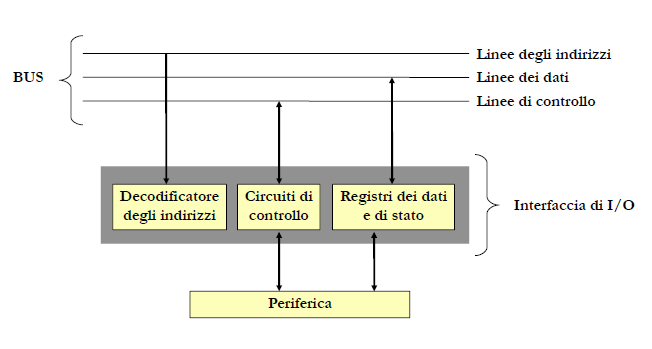
\includegraphics{./image/image-20201112230056001.png}

Comunicare con le periferiche può essere complicato, infatti se si
dovesse avere del codice per parlare con ogni singola periferica il
lavoro del programmatore diventerebbe impossibile. Per questo esiste
un'interfaccia, che fa come da traduttore tra il linguaggio della
periferica e la macchina.

E' possibile avere un interfaccia diversa per ogni periferica, ma è più
logico avere delle interfacce standard per periferiche simili. (Ad es.
USB: Universal Serial Bus).

Questa interfaccia si occupa concettualmente della gestione e dello
scambio di dati tra il processore e le periferiche. In generale
contiene:

\begin{enumerate}
\def\labelenumi{\arabic{enumi}.}
\tightlist
\item
  un registro dati della periferica
\item
  un registro di comando della periferica
\item
  un registro di stato (questo talvolta collegato al registro delle
  interruzioni del processore)
\end{enumerate}

A seconda del processore e dei registri delle periferiche, le interfacce
possono:

\begin{enumerate}
\def\labelenumi{\arabic{enumi}.}
\tightlist
\item
  condividere lo spazio di indirizzi della memoria (memory mapped I/O)
\item
  adottare uno spazio di istruzioni/indirizzi distinti (port mapped I/O)
\end{enumerate}

Le periferiche attraverso le interfacce possono essere gestite con due
metodi principalmente:

\begin{enumerate}
\def\labelenumi{\arabic{enumi}.}
\tightlist
\item
  POLLING: il processore invia sul bus il comando di lettura e si mette
  in attesa che il dato sia disponibile sul registro della periferica
  attraverso continui cicli. (PRO: facile implementazione e gestione;
  CONTRO: tiene sospeso il processore nel ciclo di attesa del dato).
\item
  INTERRUPT: il processore invia il comando di lettura alla periferica e
  poi continua le sue operazioni. Quando il dato è disponibile sul
  registro della periferica, la periferica stessa ``solleva'' un
  \emph{interrupt}, un interruzione. Il processore così interrompe le
  sue operazioni, salva il proprio stato ed esegue una opportuna routine
  per la gestione delle interruzione (compito del sistema operativo).
  Questa routine serve a verificare la presenza del dato sulla
  periferica del dato e a iniziare il trasferimento nel registro interni
  al processore, fino ad arrivare in memoria. Alla fine
  dell'\emph{interrupt} il processore ritorna alle sue operazioni
  normali. (PRO: lascia più libero il processore di operare; CONTRO:
  gestione, implementazione e controllo più complicati).
\end{enumerate}

Tra le periferiche sono presenti anche i terminali, cioè qualunque
dispositivo di puntamento (tastiera, mouse, video \ldots), e le
stampanti.

\hypertarget{architettura-software-di-un-compilatore}{%
\subsubsection{1.3) Architettura software di un
compilatore:}\label{architettura-software-di-un-compilatore}}

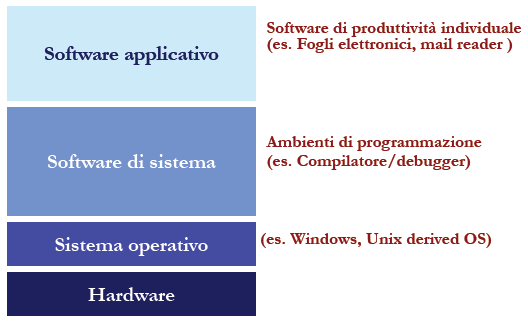
\includegraphics{./image/image-20201112231919938.png}

Con il termine \emph{sistema operativo} intendiamo l'insieme di
programmi che opera direttamente sulla macchina fisica, fornendo
interfacce di alto livello e mascherandone le caratteristiche specifiche
delle periferiche e del processore. Questo ad esempio è molto utile
nella gestione delle periferiche, perché permette di fornire un metodo
\emph{consistente} delle periferiche, ovvero una modalità standard di
interfacciarsi con le periferiche disponibili senza dover eseguire
comandi di basso livello. Importante notare inoltre che il sistema
operativo è l'unico elemento con accesso diretto alle risorse hardware,
e si riesce ad accedervi in altro modo direttamente probabilmente
abbiamo un problema.

Il sistema operativo è il modo che consente ai programmi di ottenere
risorse dal calcolatore. La traduzione da programma a calcolatore
avviene ad alto livello, in modo che non si debba scontrarsi con la
gestione degli indirizzi o dei registri. Il sistema operativo quindi,
dovendo gestire tutte le funzionalità di basso livello attraverso dei
controlli di alto livello, opera un alto livello di astrazione del
linguaggio macchina.

\hypertarget{storia-dei-sistemi-operativi}{%
\paragraph{Storia dei sistemi
operativi:}\label{storia-dei-sistemi-operativi}}

Nel 1982 Kernigham introduce Unix, prodotto dai laboratori AT\&T, che al
tempo avevano grandi esigenze di un ecosistema stabile e uguale su cui
sviluppare applicazioni. Caratteristica principale: poteva servire più
utenti contemporaneamente, usando il multitasking. Tutti gli utenti
infatti hanno un ordine di esecuzione al processore, ma sono tutti
nell'ordine del proprio utente. Da Unix poi si svilupperanno tutti i
sistemi operativi che tuttora conosciamo (Come MS-DOS o Linux).

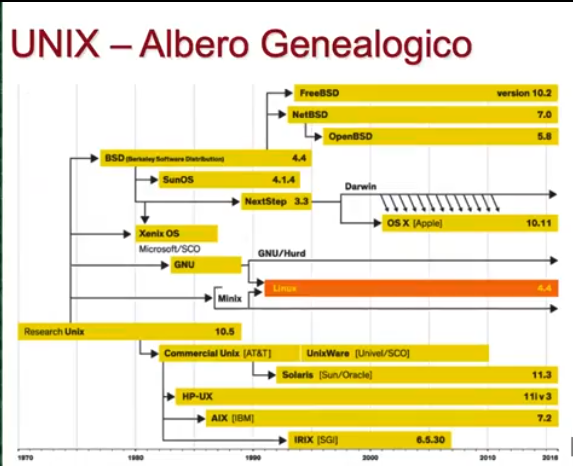
\includegraphics{./image/image-20200930171019756.png}

Architettura di un SO, che ad oggi è organizzato secondo un architettura
a \emph{strati} (anche detta \emph{onion skin architecture}). Ogni
strato fornisce un astrazione dello strato sui cui si appoggia e
permette una chiara separazione tra interfaccia e implementazione delle
diverse funzionalità, oltre che a fornire l'insieme di programmi e
librerie.

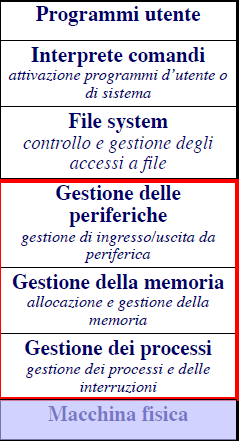
\includegraphics{./image/image-2020112323365770.png}

Il \emph{kernel} del sistema operativo, ovvero il cuore dell'OS si
occupa di:

\begin{itemize}
\tightlist
\item
  gestione periferiche (I/O informazioni)
\item
  gestione memoria (Fornisce/non fornisce al memoria in base al carico
  del momento, stabilisce il tipo di memoria da fornire)
\item
  gestione dei processi
\end{itemize}

Un processo è un entità dinamica, contrariamente al programma, infatti
viene causato dal codice in esecuzione (\emph{programma}) e dal suo
stato di esecuzione (es. valore delle sue variabili).

Un processo è quindi un insieme di due elementi:

\begin{itemize}
\tightlist
\item
  E: il codice eseguibile del programma (questo fa partire il fetch per
  creare un processo)
\item
  S: lo stato del processo
\end{itemize}

Logicamente il processo non viene gestito direttamente dal processore
reale, se no verrebbe meno il concetto di multitasking. Il processore
crea dei processori virtuali che si comportano similmente e che possono
essere assegnati a un processo.

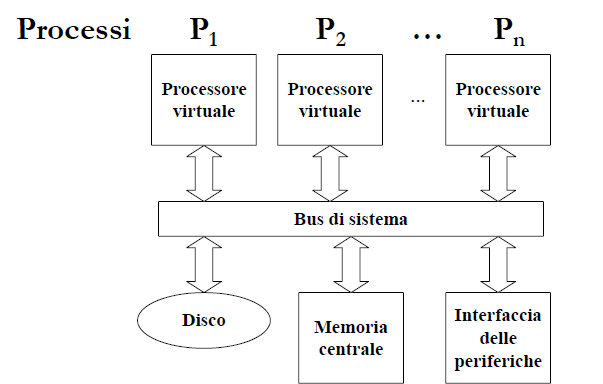
\includegraphics{./image/image-20201123234616173.png}

Nel processore è possibile che ci sia un solo processo in esecuzione in
ogni istante, mentre gli altri processi sono pronti o in attesa. Ad ogni
processo viene assegnato un valore massimo di tempo di esecuzione,
scaduto tale viene revocato il processore virtuale e assegnato a un
altro processo. Questa tecnica è detta di time-sharing, viene eseguito
dal nucleo che decide da quali processi devono andare in esecuzione
determinando lo \emph{scheduling}, che è sequenziale. La soluzione
tipica per la gestione del tempo di esecuzione di processi è a turno
(\emph{round-robin}, tutti i processi in questo hanno la stessa priorità
ad essere eseguiti, nella realtà non funziona perché alcuni processi
hanno la priorità). La CPU viene rilasciata anche quando un processo sta
aspettando un I/O da/verso una periferica.

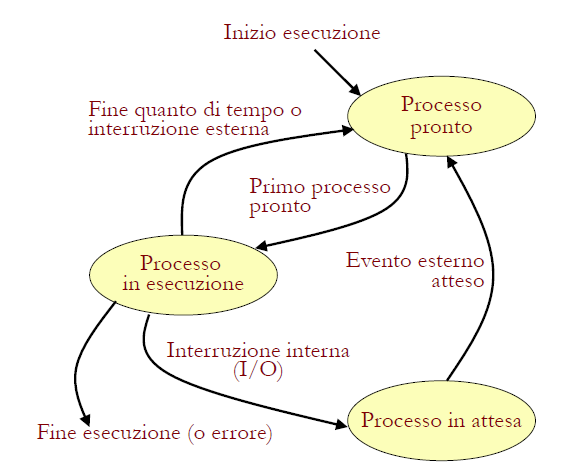
\includegraphics{./image/image-20201123235406308.png}x

In questa complicata gestione delle risorse prende parte anche la
gestione della memoria, che pensa al partizionamento della memoria tra i
vari processi che la richiedono garantendo la protezione/separazione fra
le diverse zone allocate. Il gestore memoria gestisce anche la memoria
che va assegnata ai processi, e quando i processi finisco la memoria
fisica si occupa di creare una memoria virtuale (più lenta di solito,
chiamata SWAP o semplicemente memoria virtuale) e assegnare quella
memoria.

\hypertarget{the-c-programming-language}{%
\subsection{THE C PROGRAMMING
LANGUAGE:}\label{the-c-programming-language}}

Ci sono principalmente 3 tipi di programmazione:

\begin{itemize}
\tightlist
\item
  programmazione per HARDWARE, ovvero la programmazione di dispositivi
  fisico/logici il cui il linguaggio di programmazione coincide con il
  linguaggio macchina.
\item
  programmazione per FIRMWARE, ovvero la programmazione che usa
  un'insieme comune di istruzioni mediante assembly, ovvero linguaggio
  di programmazione molto basso
\item
  programmazione per SOFTWARE, ovvero programmare in un linguaggio
  intermedio che simula le funzionalità della macchina fisica, che per
  questo permette maggiore flessibilità (nel senso che posso realizzare
  un gran numero di programmi diversi e con funzioni diverse), ma che ha
  un utilizzo delle risorse meno efficiente.
\end{itemize}

Il sistema operativo prende parte molto nell'ultimo caso, infatti è suo
il compito di fornirci le periferiche necessarie a fornire la traduzione
da linguaggio macchina (che usano ad esempio nella programmazione
firmware) e il codice. L'OS si occupa anche dell'astrazione degli
oggetti e/o delle istruzioni complesse di alto livello.

\hypertarget{diffusione-dei-linguaggi-e-perchuxe9-il-c}{%
\subsubsection{Diffusione dei linguaggi e Perché il
C}\label{diffusione-dei-linguaggi-e-perchuxe9-il-c}}

Ci sono tantissimi linguaggi di programmazione creati o utilizzati per
specifici utilizzi in cui sono molto apprezzati. Linguaggi più standard
di medio-basso livello come il C o il C++ permettono una maggior
comprensione del funzionamento della maggior parte degli altri
linguaggi, che in alcuni casi forniscono astrazioni alle strutture di
basso livello ancora presenti in questi.

Il C presenta una serie di elementi che lo rendono importante da
imparare:

\begin{itemize}
\tightlist
\item
  permette l'allocazione dinamica e altri aspetti normalmente di alto
  livello, a un livello basso.
\item
  gestione della memoria molto manuale
\item
  linguaggio apprezzato/richiesto dalle aziende
\item
  ha un astrazione che è posizionata tra il medio e il basso livello,
  motivo per cui è molto utile per ad. es. embedded system.
\end{itemize}

Il linguaggio C è stato creato nel 1972 da Kernighan e Ritchie ai Bell
Tel. Labs.

\hypertarget{operazioni-logiche-algebra-di-boole}{%
\subsubsection{1.1) Operazioni Logiche (algebra di
Boole)}\label{operazioni-logiche-algebra-di-boole}}

L'algebra di Boole è basata su tre operatori logici (NOT, AND, OR). Gli
operandi posso assumere due valori: VERO e FALSO.

Gli operatori godono della proprietà

\begin{itemize}
\tightlist
\item
  commutativa (es. A OR B = B OR A)
\item
  distributiva (es. A AND (B OR C) = (A AND B) OR (A AND C))
\end{itemize}

Le tabelle di verità associano a tutti i possibili valori degli operandi
il risultato

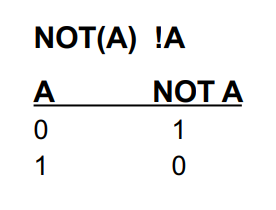
\includegraphics{./image/image-20201207220212631-1607774144622.png}

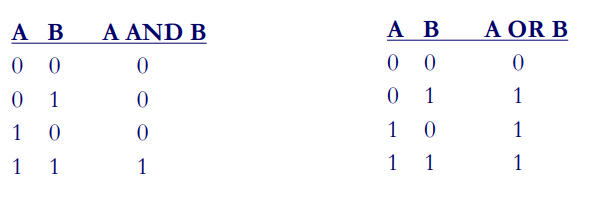
\includegraphics{./image/image-20201207220252086-1607774220882.png}

solitamente NOT viene rappresentata con !, AND con \&\& e OR con
\textbar\textbar.

quando si valuta un espressione l'ordine è il seguente (NOT, AND, OR),
per esempio.

\begin{figure}
\centering
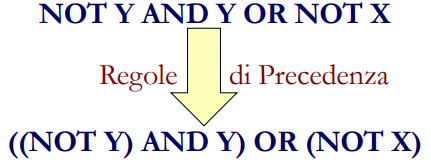
\includegraphics{C:/Users/giova/Documents/1_UNI/programmazione1/appunti/appunti-prog1/image/image-20201207220627893.png}
\caption{image-20201207220627893}
\end{figure}

Per calcolare il risultato di un espressione (per esempio NOT Y AND (Y
OR NOT X)) si crea una tabella di verità, prima con i valori singoli per
poi raggrupparli fino ad arrivare alla formula di partenza.

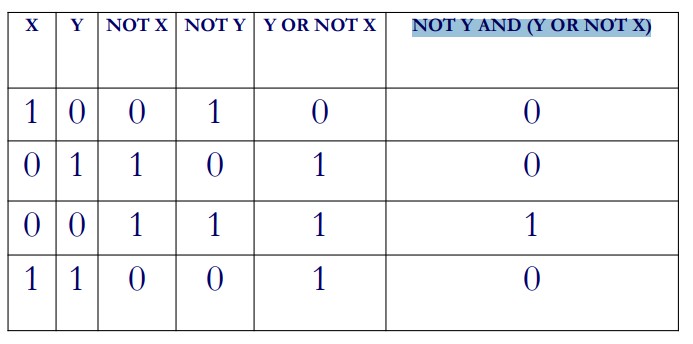
\includegraphics{./image/image-20201207220834575.png}

\hypertarget{leggi-di-de-morgan}{%
\paragraph{Leggi di De Morgan}\label{leggi-di-de-morgan}}

\begin{itemize}
\tightlist
\item
  A AND B = NOT ((NOT A) OR (NOT B))
\item
  A OR B = NOT ((NOT A) AND (NOTB))
\end{itemize}

si possono dimostrare compilando la tabella di verità e osservando che
le tabelle delle espressione ai due lati dell'uguale hanno stessi
risultati a parità di input.

\textbf{Tautologia}: espressione che è sempre vera

\textbf{Contradizione}: espressione sempre falsa

\hypertarget{codifica-semplici-algoritmi-in-c}{%
\subsubsection{1.2) Codifica Semplici Algoritmi in
C}\label{codifica-semplici-algoritmi-in-c}}

istruzione di assegnamento:

\begin{lstlisting}[language={C++}]
x = 23;
w = 'a';
y = z;
\end{lstlisting}

\hypertarget{costruttore-if-else}{%
\paragraph{Costruttore if-else}\label{costruttore-if-else}}

diagramma di flusso:

L'espressione tra parentesi viene valutata, se vera viene eseguito il
primo blocco, se falsa l'altro. Naturalmente si può utilizzare anche l'
if da solo senza else. All'interno dell'espressione posso utilizzare gli
operatori logici (\&\&, \textbar\textbar).

è sempre meglio utilizzare indentazione e paretesi graffe per una
migliore leggibilità e per non commettere errori.

\textbf{Operatore ternario ?} è un altro modo di scrivere if-else, la
sintassi è la seguente

\begin{lstlisting}[language={C++}]
espressione1 ? espressione2 : espressione3; //questo equivale al seguente if-else

if (espressione1)
    { espressione2; }
else
    { espressione3; }
\end{lstlisting}

dopo le parentesi graffe il ; non è necessario, ma se viene messo non
c'è errore.

\hypertarget{precedenza-degli-operatori}{%
\paragraph{Precedenza degli
operatori}\label{precedenza-degli-operatori}}

In un espressione vengono eseguiti prima gli operatori con precedenza
superiore, se gli operatori sono dello stesso gruppo si usano le regole
di associatività (da destra o da sinistra), le parentesi posso essere
usate per modificare la precedenza.

Associatività da sinistra a destra significa che a parità di priorità
l'espressione viene eseguita partendo da sinistra a destra.

\begin{lstlisting}[language={C++}]
if (a + b – 4 <= 9 && x < tot -1 ) // questa espressione è equivalente a quella sotto
    
if (((a + b – 4) <= 9) && (x < tot -1) )
\end{lstlisting}

\hypertarget{istruzione-iterativa-ciclo}{%
\paragraph{Istruzione Iterativa ( ciclo
)}\label{istruzione-iterativa-ciclo}}

il diagramma di flusso è il seguente (il ciclo si chiama while). Il
blocco istruzioni viene ripetuto fino a quando l'espressione non diventa
falsa.

(da pagina 38 a 56 un po' di esercizi noiosi)

\hypertarget{getchar-e-putchar}{%
\subparagraph{Getchar e Putchar}\label{getchar-e-putchar}}

\begin{lstlisting}[language={C++}]
//getchar legge il prossimo carattere inserito da tastiera
c = getchar();
//putchar stampa il carattere nello standard output
putchar(c)
\end{lstlisting}

\hypertarget{esercizio-scale}{%
\subparagraph{Esercizio scale:}\label{esercizio-scale}}

Sia data una scala di N gradini. Si supponga di salire l'intera scala
con passi da 1 , 2 o 3 scalini. In quanti possibili modi si può salire
l'intera scala ?

\textbf{risoluzione in modo semplice:}

Devo capire in quanti modi possibili posso salire una scala con n
gradini. Posso compiere passi da 1, 2 o 3 gradini.

Mi calcolo in quanti modi posso salire una scala formata da 1 2 o 3
gradini e basta.

Un gradino = 1 modo

Due gradino = 2 modo

Tre gradino = 4 modo

Per arrivare al quarto gradino ho solo tre possibilità: fare un passo da
uno, da due o da tre, quindi devo arrivare al gradino 4-1, 4-2, 4-3,
siccome so già quanti passi ci vogliono per arrivare in questi posti,
basta sommarli assieme per capire il numero di passi per arrivare al
quarto.

Aggiorno il numero di passi per il gradino n-1, n-2, n-3 e vado avanti.
(se non si capisce chiedetemi che vi spiego meglio).

\hypertarget{strutture-di-controllo}{%
\subsubsection{1.3) Strutture di
controllo}\label{strutture-di-controllo}}

\hypertarget{istruzione-di-ciclo-for}{%
\paragraph{\texorpdfstring{Istruzione di ciclo:
\emph{FOR}}{Istruzione di ciclo: FOR}}\label{istruzione-di-ciclo-for}}

schema a blocchi e sintassi:

questo operatore è utile quando so a priori quante operazioni devo fare,
in quei casi è più compatto rispetto ad un while.

\hypertarget{il-costrutto-do-while}{%
\paragraph{\texorpdfstring{Il costrutto
\emph{DO-WHILE}}{Il costrutto DO-WHILE}}\label{il-costrutto-do-while}}

schema a blocchi e sintassi:

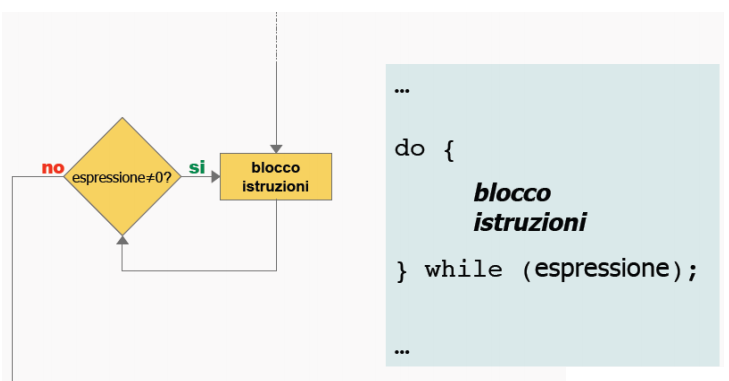
\includegraphics{./image/image-20201207224157049.png}

\begin{lstlisting}[language={C++}]
// un esempio
Contatore = 0;
do
{
    scanf (" %c", &Dato);
    Contatore ++;
} while (Dato != '%’);
\end{lstlisting}

si utilizza quando voglio eseguire un blocco di istruzioni almeno una
volta, può essere utile quando devo fare un controllo sull'input da
tastiera.

\hypertarget{il-costrutto-swith}{%
\paragraph{\texorpdfstring{Il costrutto
\emph{SWITH}}{Il costrutto SWITH}}\label{il-costrutto-swith}}

Va a sostituire un if-else multiplo, schema a blocchi e sintassi:

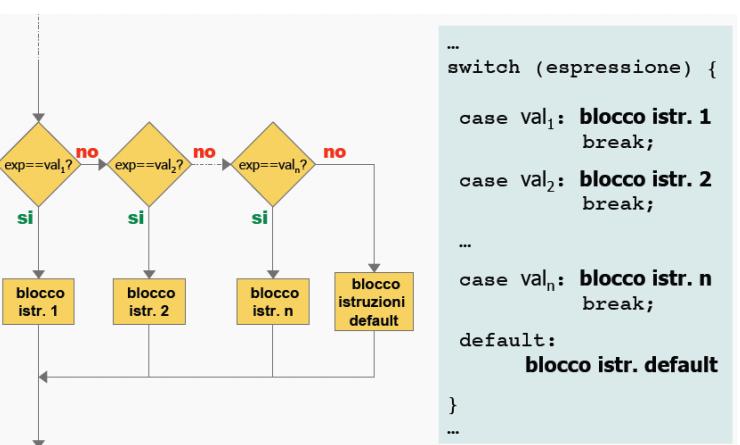
\includegraphics{./image/image-20201207224317378.png}

Il \textbf{default} (le istruzioni che vengono eseguite in caso che
nessuna delle altre sia vera) è opzionale. I singoli case vengono
eseguiti quando il valore dell'espressione è uguale a quello scritto
appena dopo l'istruzione case. ATTENZIONE: bisogna mettere il break dopo
il blocco istruzioni altrimenti si rimane all'interno dello switch
(verranno valutati i case seguenti ed eseguito il default se presente).

Valuta solo variabili di tipo INT, quindi l'espressione deve avere come
risultato un int.

\textbf{Break}: quando viene eseguito all'interno di un while, for, do,
switch provoca l'uscita dall'istruzione

\textbf{Continue}: quando viene eseguito all'interno di un ciclo passa
alla iterazione successiva

un linguaggio di programmazione può codificare qualsiasi algoritmo se
ha: sequenza di istruzioni, if-else e while.

\hypertarget{array-in-c}{%
\subsubsection{2.1) Array in C}\label{array-in-c}}

Gli array possono essere paragonati a vettori e matrici in matematica.
Da un punto di vista più concreto sono una sequenza di celle di memoria
consecutive e omogenee. L'array è quindi un contenitore per
\emph{variabili dello stesso tipo}.

A ciascun elemento dell'array si accede tramite indice (esempio a{[}i{]}
è l'elemento alla posizione i-esima). Le parentesi quadre sono operatori
ad alta precedenza (sono al primo livello della tabella).

Il primo elemento dell'array è quello in posizione 0, la macchina
astratta prende l'indice e lo somma all'indirizzo della prima cella
dell'array.

Prima di utilizzare le array bisogna dichiararle:

\begin{lstlisting}[language={C++}]
int a[100]; // dichiara un contenitore a (array) che potrà contenere 100 elementi di tipo int, il primo elemento lo si trova in a[0], l'ultimo in a[99]
\end{lstlisting}

il compilatore va a riservare la memoria per tutti questi elementi

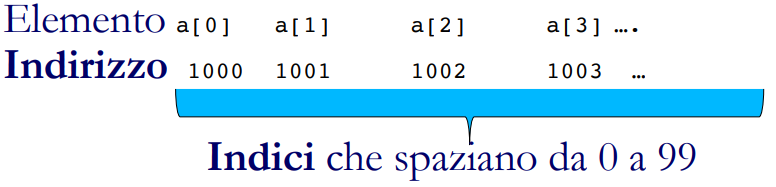
\includegraphics{./image/image-20201208144533768-1607774562526.png}

In generale l'ultimo elemento dell'array è nella posizione n-1, dove n è
la lunghezza dell'array stessa. All'interno delle parentesi si possono
mettere delle espressioni. Un veloce esercizio:

SOLUZIONE: a{[}0{]}= indeterminato, a{[}1{]} = 6

ATTENZIONE: se vado oltre l'indice massimo dell'array accedo a celle di
memoria che non appartengono all'array e il cui valore è indeterminato.

L'array in C non è un tipo, ma un costruttore di tipo.

\hypertarget{inizializzazione-e-stampa}{%
\paragraph{Inizializzazione e stampa}\label{inizializzazione-e-stampa}}

si può inizializzare direttamente al momento della dichiarazione

\begin{lstlisting}[language={C++}]
int a[5] = {5, 2, -5, 10, 234};
int b[4] = {5, 2, -5}; //un elemento non è inizializzato
int c[2] = {5, 2, -5}; // ERRORE: inizializzato un elemento che non appartiene all'array
\end{lstlisting}

per array grandi questo metodo diventa scomodo, quindi si usano i cicli
per inizializzare.

anche per stampare un array devo utilizzare un ciclo

\begin{lstlisting}[language={C++}]
printf("%d", a); // errato perchè a è un array

int i=0; // questo è il procedimento corretto
while (i<5){
    printf("%d",a[i]);
    i++;
} 
\end{lstlisting}

esercizi sulle array dalla slide 31 a 41.

\textbf{Array dinamici}: il C permette inizializzare la dimensione di un
array durante l'esecuzione di un programma (per esempio chiedendo la
dimensione da tastiera).

\hypertarget{array-multidimensionali}{%
\paragraph{Array multidimensionali}\label{array-multidimensionali}}

Le array di due dimensioni corrispondo alle matrici in matematica. Si
dichiarano nel seguente modo:

\begin{lstlisting}[language={C++}]
int a[N][M]; //N numero righe M numero colonne

//è anche possibile definire più dimensioni
int a[10][5][20];
\end{lstlisting}

Come per gli array ad 1 dimensione, anche questi possono essere
inizializzati nella fase di dichiarazione:

\begin{lstlisting}[language={C++}]
int a[4][5]= { {2, 5, -8, 7, 6},
                {3, 10, 7, 6, 1},
                {-1,8, -8, 5, 3},
                {2, 5, 8, 4, 2}
             };
\end{lstlisting}

Per semplicità possiamo immaginare l'array in due o più dimensioni, ma
la macchina astratta del C memorizza gli elementi uno dietro l'altro.
Per esempio l'array creata sopra verrà memorizzata nel seguente modo:

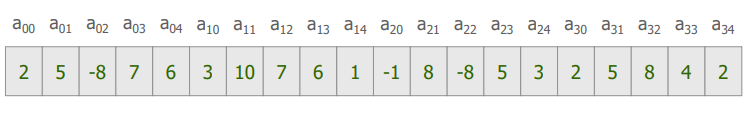
\includegraphics{./image/image-20201208150630550.png}

altri esempi di inizializzazione corretta e sbagliata:

\begin{lstlisting}[language={C++}]
int D[][]={1,2,3,4}; // errata
int E[2][]={1,2,3,4}; //errore non viene specificato il numero di colonne

int F[][4]={{1,2,3,4}}; //va bene 
// in c nella dichiarazione di un array bisogna valorizzare tutte le dimensioni, si può fare a meno di quella più a sinistra 
\end{lstlisting}

le array possono anche essere inizializzate con dei cicli

\begin{lstlisting}[language={C++}]
int main(int argc, char *argv[]){
    int matrice[10][5];
    int i=0,j=0;
    while (i<10)
    {
        j=0;
        while (j<5)
        {
            printf("%d ",matrice[i][j]);
            j++;
        }
        printf("\n");
        i++;
    }
}
\end{lstlisting}

esercizi da pagina 61 in poi

\hypertarget{stringhe-in-c}{%
\subsubsection{2.2) Stringhe in C}\label{stringhe-in-c}}

Un array di char può essere rappresentata con una stringa (per esempio
``hello''). L'ultimo carattere deve essere il carattere nullo
`\textbackslash0'. Questo carattere serve alle varie funzioni per capire
dove terminerà la stringa. Quindi quando vado a creare una stringa per
memorizzare n caratteri ne serviranno n+1 (uno lo uso per il carattere
nullo).

Esiste un modo semplificato per inizializzare un'array di caratteri come
stringa:

\begin{lstlisting}[language={C++}]
char mia_stringa[] = “Ciao a tutti!”;
\end{lstlisting}

Questo mi memorizza automaticamente lo spazio per il miei caratteri più
il carattere terminatore. Quindi il risultato sarà:

\begin{figure}
\centering
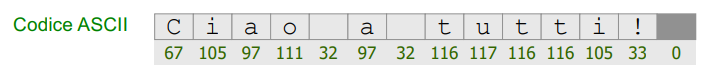
\includegraphics{C:/Users/giova/Documents/1_UNI/programmazione1/appunti/appunti-prog1/image/image-20201212103116117.png}
\caption{image-20201212103116117}
\end{figure}

L'inizializzazione vista sopra è molto più veloce ed è equivalente ad
inizializzare nel seguente modo:

\begin{lstlisting}[language={C++}]
char mia_stringa[] = {‘C’,‘i’,‘a’,’o’,’ ‘,’a’,’ ‘,’t’,’u’,’t’,’t’,’i’,’!’,’\0’};
\end{lstlisting}

Se non specifico il numero all'interno delle parentesi quadre quando
dichiaro l'array il compilatore va a riservare uno spazio pari al numero
degli elementi con cui l'array viene inizializzato. Nel caso delle
stringhe posso anche dichiarare esplicitamente la dimensione di memoria
da riservare:

\begin{lstlisting}[language={C++}]
char frase[20]=”Ciao a tutti!”;
\end{lstlisting}

Bisogna stare attenti che un elemento (dei 20 messi a disposizione per
l'array) sarà occupato da `\textbackslash0' e poi gli elementi in più
saranno lasciati vuoti.

ATTENZIONE: se non specifico né il numero di caratteri (all'interno
delle parentesi quadre) né assegno alla stringa un valore, il
compilatore da un errore, perché non sa quanta memoria riservare.

\begin{lstlisting}
char parola[]; // ERRORE
\end{lstlisting}

per stampa le stringhe si usa \%s:

\begin{lstlisting}[language={C++}]
printf(“%s”, mia_stringa); //questo non sarebbe possibile se non ci fosse il carattere terminatore perché non saprei dove fermarmi 
\end{lstlisting}

quando faccio scanf non bisogna mettere la \& perché la stringa è un
array e la variabile con il suo nome è già un indirizzo.

\begin{lstlisting}[language={C++}]
scanf(“%s”, parola);
\end{lstlisting}

\hypertarget{rappresentazione-di-informazioni}{%
\subsubsection{2.4) Rappresentazione di
informazioni}\label{rappresentazione-di-informazioni}}

in un calcolatore le informazioni vengono rappresentate sotto forma di
dati, codificati in un linguaggio comprensibile al calcolatore. Per
permetterci di interpretare le informazioni i dati devono essere
decodificati. Quindi ci sono diversi livelli di decodifica che partono
dall'hardware fino ad arrivare ad informazioni interpretabili a noi
umani.

I tipi di dato che il calcolatore può interpretare direttamente sono :

\begin{itemize}
\tightlist
\item
  booleani
\item
  numeri interi
\item
  numeri frazionari
\item
  caratteri
\end{itemize}

Per questi dati la codifica è gestita direttamente dall'HW, per tipi di
dato più complessi si usa una rappresentazione di tipo software.

\hypertarget{interi}{%
\paragraph{Interi}\label{interi}}

Sono rappresentati da una sequenza finita di bit. 8 bit (un byte)
permettono di rappresentare i valori da 0 a 255. Solitamente per gli
interi positivi si usano 4 byte (32 bit), quindi i numeri vanno da 0 a
4.294.967.295. (questo implica che all'interno dei calcolatori i numeri
sono finiti).

Per rappresentare anche i numeri negativi, si utilizza il primo bit come
bit di segno (0 per i numeri negativi, 1 per i positivi)

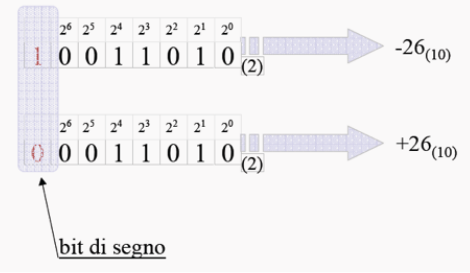
\includegraphics{./image/image-20201212110945997.png}

In realtà nei calcolatori non si usa questa rappresentazione ma quella
in complemento a due con i seguenti vantaggi: non c'è un doppio zero,
non c'è bisogno di una circuiteria specifica. Esempio:

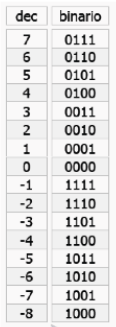
\includegraphics{./image/image-20201212111232217.png}

Per decodificare i valori positivi si procede nel modo normale, per
quelli negativi si decodifica e poi si sottrae 2\^{}N-1. Per invertire i
numeri si invertono gli zeri con gli uno e si somma uno.

\hypertarget{numeri-frazionari}{%
\subparagraph{Numeri frazionari}\label{numeri-frazionari}}

I dati con numeri dopo la virgola vanno rappresentati in maniera
opportuna, ci sono due tecniche:

\begin{itemize}
\tightlist
\item
  \textbf{virgola fissa}: si dividono i bit che rappresentano i valori
  interi da quello per i valori dopo la virgola
\item
  \textbf{virgola mobile}: la maggior parte dei bit viene usata per le
  cifre rappresentative del numero, gli altri per sapere dove mettere la
  virgola.
\end{itemize}

esempio codifica virgola fissa:

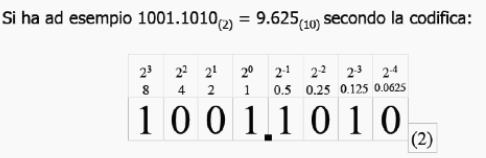
\includegraphics{./image/image-20201212112345743.png}

Per la virgola mobile solitamente vengono utilizzati 32 bit, 1 per il
segno, 8 per l'esponente e il resto per la mantissa

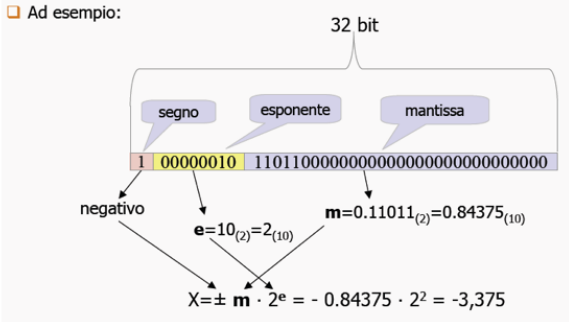
\includegraphics{./image/image-20201212112608865.png}

Quindi la mantissa rappresenta numeri da 0 a 1, che verranno
moltiplicati per 2\^{}e in modo da ottenere il numero desiderato. \[
m=0.11011_{(2)} =  2^{-1}+2^{-2}+2^{-4}+2^{-5} = 0.84375
\] un numero si dice normalizzato se l'esponente è diverso da 0, la
mantissa è compresa tra 1 e 2 l'intervallo dei numeri è \[
(-2^{128}, -2^{-126}][2^{-126}, 2^{128})
\]

\hypertarget{caratteri}{%
\subparagraph{Caratteri}\label{caratteri}}

per codificare i caratteri si utilizza la tabella ASCII, i primi 128
valori sono fissi i successivi rappresentato la tabella ASCII estesa con
caratteri più specifici (per esempio c'è una tabella ASCII estesa con i
caratteri è, ò, à\ldots).

attualmente si utilizza l'UNICODE che utilizza 2 bytes per ogni
carattere e permette di non avere tabelle diverse per ogni regione del
mondo.

\end{document}
